\documentclass[12pt,a4paper]{article}
\usepackage[utf8]{inputenc}
\usepackage{graphicx}
%\usepackage[T1]{fontenc}
\usepackage[T2A]{fontenc}
\usepackage{indentfirst}
\usepackage{hyperref}
\usepackage{blindtext}
\usepackage{xcolor}
\graphicspath{{img/}}
\hypersetup{
  colorlinks,
  linkcolor={black},
  citecolor={black},
  urlcolor={black}
}
\usepackage{listings}
\usepackage{color}
\usepackage{cmap}
\renewcommand{\rmdefault}{ftm}
\definecolor{dkgreen}{rgb}{0,0.6,0}
\definecolor{gray}{rgb}{0.5,0.5,0.5}
\definecolor{mauve}{rgb}{0.58,0,0.82}

\lstset{frame=tb,
  language=Java,
  aboveskip=3mm,
  belowskip=3mm,
  showstringspaces=false,
  columns=flexible,
  basicstyle={\small\ttfamily},
  numbers=none,
  numberstyle=\tiny\color{gray},
  keywordstyle=\color{blue},
  commentstyle=\color{dkgreen},
  stringstyle=\color{mauve},
  breaklines=true,
  breakatwhitespace=true,
  tabsize=3
}
%Hyphenation rules
%--------------------------------------
\usepackage{hyphenat}
\hyphenation{ма-те-ма-ти-ка вос-ста-нав-ли-вать}
%--------------------------------------
\usepackage[english,russian]{babel}
\title{Название}

\begin{document}
\maketitle
\tableofcontents
\pagebreak

\section{Глава 1. Название главы}
\subsection{Операции над множествами.}

\begin{enumerate}
    \item Объединение 
      \[A \cup B=\{x|x \in A \lor x\in B\}\]
    \begin{center}   
      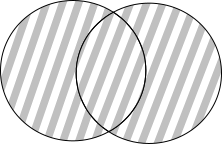
\includegraphics[scale=0.65]{bitmap.png}
    \end{center}
  \end{enumerate}

\subsection{Понятие класса.}

Класс - чертеж объекта, основа из чего будет создаваться объект. Определяет какие атрибуты и методы будут принадлежать все его объектам.

\begin{lstlisting}
public class ClassTwo {
    private String name;

    public String getName() {
        return name;
    }
 
    public void setName(String name) {
        this.name = name;
    } 
}

\end{lstlisting}

\end{document}
